\paragraph{複屈折(1軸性結晶)}
1軸異方性の場合を考えよう.1軸性結晶には菱面体晶系,正方晶系,六方晶系などがある.
光学軸を$\zeta$軸とし,
\begin{align}
  \varepsilon=
  \begin{pmatrix}
    \varepsilon_{\text T} & 0 & 0\\
    0 & \varepsilon_{\text T} & 0\\
    0 & 0 & \varepsilon_{\text P}
  \end{pmatrix}
  \label{uniaxial_tensor1}
\end{align}
とする.この時,Fresnel方程式は因数分解され,
\begin{align}
  \dfrac{1}{\varepsilon_0}=\mu{c}^2&=\dfrac{n^2}{\varepsilon_{\text T}}\label{uniaxial_ordinary}\\
  \dfrac{1}{\varepsilon_0}=\mu{c}^2&=\dfrac{{n_\xi}^2+{n_\eta}^2}{\varepsilon_{\text P}}+\dfrac{{n_\zeta}^2}{\varepsilon_{\text T}}\label{uniaxial_extraordinary}
\end{align}
となる.(\ref{uniaxial_ordinary})を常光線,(\ref{uniaxial_extraordinary})を異常光線と言う.
Fresnel方程式は$(n_\xi,n_\eta,n_\zeta)$空間において,4次曲面を描くのであった.
これが因数分解されるといことは,曲面が2つ存在するということである.
それらが常光線と異常光線である.
常光線(\ref{uniaxial_ordinary})は球を,異常光線(\ref{uniaxial_extraordinary})は回転楕円体を表す.
これらを図示すると,以下のようになる($\varepsilon_{\text T}$と$\varepsilon_{\text P}$の大小で2通りに分かれる).

\begin{figure}[ht]
  \centering
  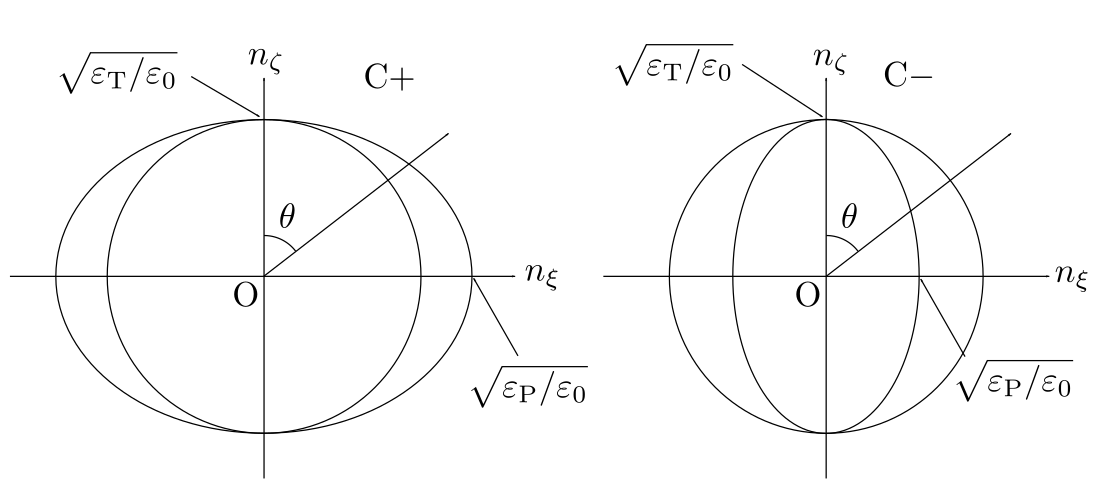
\includegraphics[scale=0.35]{uniaxiNvec.pdf}
  \caption{正結晶(左)と負結晶(右)}
  \label{uniaxiNvec}
\end{figure}

正結晶には水晶,氷;負結晶には方解石,ADPなどがある.
中心から$\boldsymbol{n}$の方向に引いた線分と曲面の交点が2つの屈折率ベクトルとなる.
異方性媒質一般で見たように,
光線ベクトルはFresnel方程式から決定される屈折率ベクトル面の法線の向きを向いているのであった.
なので,常光線においては$\boldsymbol{s}$と$\boldsymbol{n}$の向きは一致する.これは$\boldsymbol{E}$と$\boldsymbol{D}$の向きも一致するということである.
\eqref{aniso_newD}からも分かるように,
\begin{align}
  \boldsymbol{D}=\dfrac{1}{\mu{c^2}}n^2\boldsymbol{E}=\varepsilon_{\text T}\boldsymbol{E}
\end{align}
となる.つまり,
常光線は等方的な誘電率$\varepsilon_{\text T}$を持つ媒質中の光と同じように振る舞うことが分かる.

異常光線においても,光線ベクトルは屈折率ベクトル面の法線の向きを向いていることを考慮すると,
光線ベクトル$\boldsymbol{s}$は光学軸と屈折率ベクトル$\boldsymbol{n}$を通る平面(主断面)内に存在することが分かる.
$\boldsymbol{n}$が光学軸となす角を$\theta$とすると,(\ref{uniaxial_extraordinary})から,
\begin{align}
  \dfrac{1}{n^2}=\dfrac{\varepsilon_0}{\varepsilon_{\text P}}\sin^2\theta+\dfrac{\varepsilon_0}{\varepsilon_{\text T}}\cos^2\theta
\end{align}
となる.簡単のため,$\boldsymbol{n}$が$\xi\zeta$平面に存在するものとする.
この時,半直線と楕円の交点における法線の方向(光線ベクトルの向きに等しい)は,
\[\left(\dfrac{\tan\theta}{\varepsilon_{\text P}},0,\dfrac{1}{\varepsilon_{\text T}}\right)\]
となる.光線ベクトルが光学軸となす角$\theta'$は一般の場合に戻して考えても結局,
\begin{align}
  \tan\theta'=\dfrac{\varepsilon_{\text T}}{\varepsilon_{\text P}}\tan\theta\label{uniaxial_sandn}
\end{align}
である.$\boldsymbol{n}$が$\boldsymbol{s}$と同じ向きを向くのは,光学軸に平行に伝わる場合か,垂直に伝わる場合のみである.

以上の事実を踏まえれば常光線と以上光線の電場と磁場,そして磁束密度の位置関係が分かる.
異方性媒質中では2つの光波は直線偏光であることに注意.
まずは屈折率楕円体を考えよう.
この座標系では,屈折率楕円体は回転楕円体となる.それは次に示すようになる.

\begin{figure}[ht]
  \centering
  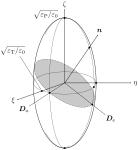
\includegraphics[scale=0.4]{uniaxial_nEllipse.pdf}
  \caption{常光線と異常光線の電束密度を示す屈折率楕円体(正結晶)}
  \label{uniaxial_nEllipse}
\end{figure}

以後,断りがないかぎり常光線の物理量を添字$_{\text o}$,異常光線の物理量を添字$_{\text e}$で表す.
屈折率楕円体からは2つの電束密度が存在することしか分からないが,(\ref{uniaxial_ordinary})を見れば,楕円の主半径のうち,$\zeta=0$に存在する方が常光線だと分かる.
以上の考察から重要な結果が得られた.
まず,常光線の電束密度は$\xi\eta$平面上に存在するということである.
もう一つが異常光線ベクトルの電束密度は主断面上に存在するということである.
常光線においては光は誘電率$\varepsilon_{\text T}$の等方的な媒質中と同じように振舞うので,常光線の電場は$\xi\eta$平面に存在することが分かる.
さらに,$\boldsymbol{E},\boldsymbol{D},\boldsymbol{s},\boldsymbol{n}$は同一平面内に存在するので,異常光線の電場は主断面上に存在することが分かる.
磁場の方向については,$\boldsymbol{H}=\dfrac{1}{\omega\mu}\boldsymbol{n}\times\boldsymbol{E}$から簡単に導くことができよう.

以上から,常光線と異常光線の電場と磁場の方向を図示すると本文図8-13のようになる.

1軸性の異方性を持つ媒質中では光はこのように進む.この2つの光は直線偏光である.

これまでは異方的な媒質の中のみを進む光を考えてきた.ここで,異方的な媒質に入る光について考えてみよう.
境界面を$y=0$,光学軸を$z$軸に取る.入射前の$\boldsymbol{n}$は$yz$平面に存在していたとする.
真空中から角度$\theta$で入射した光は異方性媒質に入ると常光線と異常光線に分かれる.
常光線の屈折角$\theta$は
\begin{align}
  \sqrt{\varepsilon_0}\sin\theta=\sqrt{\varepsilon_{\text T}}\sin\theta_{\text o}\label{uniaxial_refo}
\end{align}
で与えられる.異常光線の屈折角は(\ref{uniaxial_extraordinary})と(\ref{uniaxial_sandn})から,
\begin{align}
  \tan\theta_{\text e}=\sqrt{\dfrac{\varepsilon_{\text P}\varepsilon_0}{\varepsilon_{\text T}\left(\varepsilon_{\text T}-\varepsilon_0\sin^2\theta\right)}}\sin\theta\label{uniaxial_refe}
\end{align}
で与えられる.我々が光の進む向きとして観測するのは波数や位相速度の向きでなく,群速度の向きである.
(\ref{uniaxial_refo})と(\ref{uniaxial_refe})から,常光線と異常光線は屈折角が異なる.
そのため,1軸性異方性媒質を特定の条件で通った光は,別々の光線に分かれる.これを複屈折と呼ぶ.

\paragraph{円錐屈折(2軸性結晶)}
2軸性異方性媒質ではテンソル$\varepsilon$の主値は全て異なる.2軸性結晶には三斜晶系,単斜晶系,菱面体晶系などがある.
以下では,テンソルの主値を
\begin{align}
  \varepsilon_\xi < \varepsilon_\eta < \varepsilon_\zeta\label{biaxial_nlarge}
\end{align}
とする.このようにしても一般性を失わないことは明らかである.
Fresnel方程式は,
\begin{align}
  n^2\left(\varepsilon_{\xi}{n_\xi}^2+\varepsilon_{\eta}{n_\eta}^2+\varepsilon_{\zeta}{n_\zeta}^2\right)
  -\mu{c}^2\left[{n_\xi}^2\varepsilon_\xi(\varepsilon_\eta+\varepsilon_\zeta)
  +{n_\eta}^2\varepsilon_\eta(\varepsilon_\zeta+\varepsilon_\xi)
  +{n_\zeta}^2\varepsilon_\zeta(\varepsilon_\eta+\varepsilon_\xi)\right]
  +\mu^2{c}^4\varepsilon_\xi\varepsilon_\eta\varepsilon_\zeta=0\label{biaxial_fresEq}
\end{align}
のように書けるのであった.まずはこの4次曲面,つまり屈折率ベクトル面の形状を求めよう.
$n_\xi{}n_\eta$平面での切り口は,(\ref{biaxial_fresEq})に$n_\zeta=0$を代入して,
\[\left(n^2-\mu{c^2}\varepsilon_\zeta\right)\left(\varepsilon_\xi{n_\xi}^2+\varepsilon_\eta{n_\eta}^2-\mu{c^2}\varepsilon_\xi\varepsilon_\eta\right)=0\]
より,円
\begin{align}
  \dfrac{{n_\xi}^2}{\varepsilon_\zeta/\varepsilon_0}+\dfrac{{n_\eta}^2}{\varepsilon_\zeta/\varepsilon_0}=1
\end{align}
及び楕円
\begin{align}
  \dfrac{{n_\xi}^2}{\varepsilon_\eta/\varepsilon_0}+\dfrac{{n_\eta}^2}{\varepsilon_\xi/\varepsilon_0}=1
\end{align}
となる.(\ref{biaxial_nlarge})の条件から,楕円は円の内側にあることが分かる.
同様に計算すると,
\begin{align}
  \dfrac{{n_\eta}^2}{\varepsilon_\xi/\varepsilon_0}+\dfrac{{n_\zeta}^2}{\varepsilon_\xi/\varepsilon_0}=1\\
  \dfrac{{n_\eta}^2}{\varepsilon_\zeta/\varepsilon_0}+\dfrac{{n_\zeta}^2}{\varepsilon_\eta/\varepsilon_0}=1\\
  \dfrac{{n_\zeta}^2}{\varepsilon_\eta/\varepsilon_0}+\dfrac{{n_\xi}^2}{\varepsilon_\eta/\varepsilon_0}=1\label{biaxial_xzc}\\
  \dfrac{{n_\zeta}^2}{\varepsilon_\xi/\varepsilon_0}+\dfrac{{n_\xi}^2}{\varepsilon_\zeta/\varepsilon_0}=1\label{biaxial_xze}
\end{align}
が得られる.これらを図示すると,次のようになる.

\begin{figure}[ht]
  \centering
  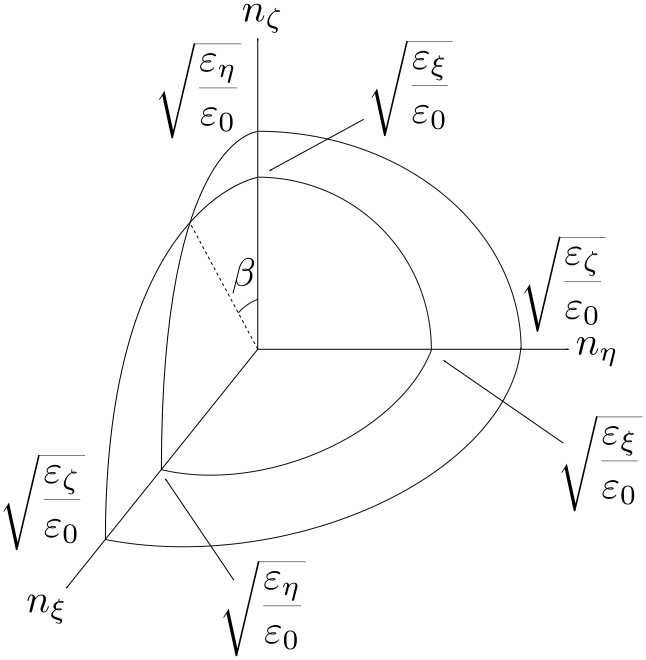
\includegraphics[scale=0.35]{fresnel.pdf}
  \caption{}
  \label{fresnel}
\end{figure}

この曲面は自身との交点を4つ持っており,それらは$n_\xi{}n_\zeta$平面の各象限に存在する.
特異点の傾き$\beta$は,(\ref{biaxial_xzc})と(\ref{biaxial_xze})から,
\begin{align}
  \tan\beta=\pm\sqrt{\dfrac{\varepsilon_\zeta(\varepsilon_\eta-\varepsilon_\xi)}{\varepsilon_\xi(\varepsilon_\zeta-\varepsilon_\eta)}}\label{biaxial_betat}\\
  \cos\beta=\pm\sqrt{\dfrac{\varepsilon_\xi(\varepsilon_\zeta-\varepsilon_\eta)}{\varepsilon_\eta(\varepsilon_\zeta-\varepsilon_\xi)}}\label{biaxial_betac}\\
  \sin\beta=\pm\sqrt{\dfrac{\varepsilon_\zeta(\varepsilon_\eta-\varepsilon_\xi)}{\varepsilon_\eta(\varepsilon_\zeta-\varepsilon_\xi)}}\label{biaxial_betas}
\end{align}
で与えられる.この式により,$n_\xi{}n_\zeta$平面上に2本の軸が決定される.
2軸性異方性媒質ではこの軸のことを光学軸もしくは双法線と呼ぶ.
光学軸の方向は,波動ベクトルの絶対値が一つの値しか取らない,つまりFresnel方程式が重解を持つ方向である.
また,$n$の値が1つに定まることから,光学軸の向きで屈折率楕円体を切断すると断面は円となる.

光線ベクトルと光線速度面についても同様の式が成り立つ.
光線速度面方程式は,
\begin{align}
  s^2\left(\varepsilon_\eta\varepsilon_\zeta{s_\xi}^2 + \varepsilon_\zeta\varepsilon_\xi{s_\eta}^2 + \varepsilon_\xi\varepsilon_\eta{s_\zeta}^2\right)
  -\dfrac{1}{\mu{}c^2}\left[{s_\xi}^2(\varepsilon_\eta+\varepsilon_\zeta)+{s_\eta}^2(\varepsilon_\zeta+\varepsilon_\xi)+{s_\zeta}^2(\varepsilon_\xi+\varepsilon_\eta)\right]
  +\dfrac{1}{\mu^2c^4}=0
\end{align}
で与えられるのであった.これも,$s$座標系で4次曲面をなす.特異点が$\zeta$軸となす角を$\gamma$とする.
\begin{align}
  \dfrac{{s_\zeta}^2}{\varepsilon_0/\varepsilon_\eta}+\dfrac{{s_\xi}^2}{\varepsilon_0/\varepsilon_\eta}=1\label{biaxial_szxc}\\
  \dfrac{{s_\zeta}^2}{\varepsilon_0/\varepsilon_\xi}+\dfrac{{s_\xi}^2}{\varepsilon_0/\varepsilon_\zeta}=1\label{biaxial_szxe}
\end{align}
から,
\begin{align}
  \tan\gamma=\pm\sqrt{\dfrac{\varepsilon_\eta-\varepsilon_\xi}{\varepsilon_\zeta-\varepsilon_\eta}}=\sqrt{\dfrac{\varepsilon_\zeta}{\varepsilon_\xi}}\tan\beta\label{biaxial_gamma}
\end{align}
となる.最後の式変形には(\ref{biaxial_betat})を使った.この$\gamma$で決定される2本の軸を光線軸もしくは双径線と呼ぶ.
また,$s$の値が1つに定まることから,光線軸の向きでFresnel楕円体を切断すると断面は円となる.
さらに,(\ref{biaxial_nlarge}),(\ref{biaxial_gamma})から,
\begin{align}
  \gamma < \beta
\end{align}
であることが分かる.

異方性媒質一般で調べたように,$\boldsymbol{s}$は屈折率ベクトル面の法線方向を向くのであった.
つまり,
\begin{align}
  \dfrac{\partial f}{\partial\boldsymbol{n}}\parallel\boldsymbol{s}\label{biaxial_fns}
\end{align}
である.(\ref{biaxial_fresEq})から,
\begin{align}
  \begin{split}
    An_\xi\left[\mu{c^2}\varepsilon_\xi(\varepsilon_\eta+\varepsilon_\zeta)-\varepsilon_\xi{n^2}-(\varepsilon_{\xi}{n_\xi}^2+\varepsilon_{\eta}{n_\eta}^2+\varepsilon_{\zeta}{n_\zeta}^2)\right]=s_\xi\\
    An_\eta\left[\mu{c^2}\varepsilon_\eta(\varepsilon_\zeta+\varepsilon_\xi)-\varepsilon_\eta{n^2}-(\varepsilon_{\xi}{n_\xi}^2+\varepsilon_{\eta}{n_\eta}^2+\varepsilon_{\zeta}{n_\zeta}^2)\right]=s_\eta\\
    An_\zeta\left[\mu{c^2}\varepsilon_\zeta(\varepsilon_\xi+\varepsilon_\eta)-\varepsilon_\zeta{n^2}-(\varepsilon_{\xi}{n_\xi}^2+\varepsilon_{\eta}{n_\eta}^2+\varepsilon_{\zeta}{n_\zeta}^2)\right]=s_\zeta
  \end{split}\label{biaxial_ns}
\end{align}
となれば良い.ただし,$A$は0でない定数である.
$\boldsymbol{s}$と$\boldsymbol{n}$が平行になるのは,誘電主軸の向きに伝播する時のみだと分かる.
$\boldsymbol{s}$は群速度の向きを向いていて,大きさが$\boldsymbol{s}\cdot\boldsymbol{n}=1$で決定されるのであった.(\ref{biaxial_ns})から,
\begin{align*}
  & A{n_\xi}^2\left[\mu{c^2}\varepsilon_\xi(\varepsilon_\eta+\varepsilon_\zeta)-\varepsilon_\xi{n^2}-(\varepsilon_{\xi}{n_\xi}^2+\varepsilon_{\eta}{n_\eta}^2+\varepsilon_{\zeta}{n_\zeta}^2)\right]\\
  &+ A{n_\eta}^2\left[\mu{c^2}\varepsilon_\eta(\varepsilon_\zeta+\varepsilon_\xi)-\varepsilon_\eta{n^2}-(\varepsilon_{\xi}{n_\xi}^2+\varepsilon_{\eta}{n_\eta}^2+\varepsilon_{\zeta}{n_\zeta}^2)\right]\\
  &+ A{n_\zeta}^2\left[\mu{c^2}\varepsilon_\zeta(\varepsilon_\xi+\varepsilon_\eta)-\varepsilon_\zeta{n^2}-(\varepsilon_{\xi}{n_\xi}^2+\varepsilon_{\eta}{n_\eta}^2+\varepsilon_{\zeta}{n_\zeta}^2)\right]=1
\end{align*}
となるので,これを解くと,
\begin{align}
  A=\dfrac{\varepsilon_0}{{n_\xi}^2\varepsilon_\xi\left(\varepsilon_\eta+\varepsilon_\zeta\right)+{n_\eta}^2\varepsilon_\eta\left(\varepsilon_\zeta+\varepsilon_\xi\right)+{n_\zeta}^2\varepsilon_\zeta\left(\varepsilon_\xi+\varepsilon_\eta\right)-2\varepsilon_0n^2\left(\varepsilon_{\xi}{n_\xi}^2+\varepsilon_{\eta}{n_\eta}^2+\varepsilon_{\zeta}{n_\zeta}^2\right)}
\end{align}
となる.(\ref{biaxial_ns})に代入すると,
\begin{align}
  \begin{split}
    s_\xi=\dfrac{n_\xi\left[\varepsilon_\xi(\varepsilon_\eta+\varepsilon_\zeta)-\varepsilon_0\varepsilon_\xi{n^2}-\varepsilon_0(\varepsilon_{\xi}{n_\xi}^2+\varepsilon_{\eta}{n_\eta}^2+\varepsilon_{\zeta}{n_\zeta}^2)\right]}
    {{n_\xi}^2\varepsilon_\xi\left(\varepsilon_\eta+\varepsilon_\zeta\right)+{n_\eta}^2\varepsilon_\eta\left(\varepsilon_\zeta+\varepsilon_\xi\right)+{n_\zeta}^2\varepsilon_\zeta\left(\varepsilon_\xi+\varepsilon_\eta\right)-2\varepsilon_0n^2\left(\varepsilon_{\xi}{n_\xi}^2+\varepsilon_{\eta}{n_\eta}^2+\varepsilon_{\zeta}{n_\zeta}^2\right)}\\
    %
    s_\eta=\dfrac{n_\eta\left[\varepsilon_\eta(\varepsilon_\zeta+\varepsilon_\xi)-\varepsilon_0\varepsilon_\eta{n^2}-\varepsilon_0(\varepsilon_{\xi}{n_\xi}^2+\varepsilon_{\eta}{n_\eta}^2+\varepsilon_{\zeta}{n_\zeta}^2)\right]}
    {{n_\xi}^2\varepsilon_\xi\left(\varepsilon_\eta+\varepsilon_\zeta\right)+{n_\eta}^2\varepsilon_\eta\left(\varepsilon_\zeta+\varepsilon_\xi\right)+{n_\zeta}^2\varepsilon_\zeta\left(\varepsilon_\xi+\varepsilon_\eta\right)-2\varepsilon_0n^2\left(\varepsilon_{\xi}{n_\xi}^2+\varepsilon_{\eta}{n_\eta}^2+\varepsilon_{\zeta}{n_\zeta}^2\right)}\\
    %
    s_\zeta=\dfrac{n_\zeta\left[\varepsilon_\zeta(\varepsilon_\xi+\varepsilon_\eta)-\varepsilon_0\varepsilon_\zeta{n^2}-\varepsilon_0(\varepsilon_{\xi}{n_\xi}^2+\varepsilon_{\eta}{n_\eta}^2+\varepsilon_{\zeta}{n_\zeta}^2)\right]}
    {{n_\xi}^2\varepsilon_\xi\left(\varepsilon_\eta+\varepsilon_\zeta\right)+{n_\eta}^2\varepsilon_\eta\left(\varepsilon_\zeta+\varepsilon_\xi\right)+{n_\zeta}^2\varepsilon_\zeta\left(\varepsilon_\xi+\varepsilon_\eta\right)-2\varepsilon_0n^2\left(\varepsilon_{\xi}{n_\xi}^2+\varepsilon_{\eta}{n_\eta}^2+\varepsilon_{\zeta}{n_\zeta}^2\right)}
  \end{split}
  \label{biaxial_ncomp}
\end{align}
が得られる.$\boldsymbol{n}$が双法線の向きを向いている場合を考えよう.この時,$\boldsymbol{n}$は曲面$f=0$の特異点を通る.
この方程式はこの点において重解をもつので,特異点における$\dfrac{\partial{f}}{\partial{n_i}}$は0である.
この時,(\ref{biaxial_ncomp})は$0/0$の不定形になる.よって,双法線方向に進む光については別に考え直す必要がある.

まずは,ある座標系に屈折率ベクトル面と光線速度面を作ろう(これらはFresnel方程式,光線速度面方程式から決定され,異なる座標系に属するものだが,適当な目盛で両者の空間を一致させたとする).
これを今までに習い$(\xi,\eta,\zeta)$空間とし,$\xi\eta$平面を図示すると次のようになる(屈折率ベクトル面を考える際は$i\to{}n_i$,光線速度面を考える際は$i\to{}s_i$と書き換える).

\begin{figure}[ht]
  \centering
  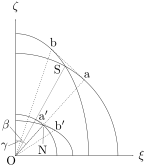
\includegraphics[scale=0.35]{biaxinands.pdf}
  \caption{}
  \label{biaxinands}
\end{figure}

まずは光線速度面Sに2点で接する直線abを求めよう.(\ref{biaxial_betat}),(\ref{biaxial_szxc}),(\ref{biaxial_szxe})から,これは
\begin{align}
  s_\xi\sin\beta+s_\zeta\cos\beta=\sqrt{\dfrac{\varepsilon_0}{\varepsilon_\eta}}
\end{align}
となる.さらにOaが$\zeta$軸となす角は,aが半径$\sqrt{\varepsilon_0/\varepsilon_\eta}$の円周上だということを考えると,$\beta$である.
よって,屈折率ベクトル面の特異点Nと原点を通る直線と光線速度面との交点は,光線速度面とある直線の接点であり,この直線は法線となる.
次に,これを三次元に拡張しよう.光線速度面の方程式は,
\begin{align}
  g & = \left({s_\xi}^2+{s_\eta}^2+{s_\zeta}^2\right)\left(\varepsilon_\eta\varepsilon_\zeta{s_\xi}^2+\varepsilon_\zeta\varepsilon_\xi{s_\eta}^2+\varepsilon_\xi\varepsilon_\eta{s_\zeta}^2\right) \notag \\
  &-{\varepsilon_0}\left[{s_\xi}^2(\varepsilon_\eta+\varepsilon_\zeta)+{s_\eta}^2(\varepsilon_\zeta+\varepsilon_\xi)+{s_\zeta}^2(\varepsilon_\xi+\varepsilon_\eta)\right]
  +{\varepsilon_0}^2=0\label{biaxial_g0}
\end{align}
である.さらに,これの$\boldsymbol{a}(\sqrt{\varepsilon_0/\varepsilon_\eta}\sin\beta,0,\sqrt{\varepsilon_0/\varepsilon_\eta}\cos\beta)$での接平面は,
\begin{align*}
  \dfrac{\partial{g}}{\partial\boldsymbol{s}}(\boldsymbol{a})\cdot(\boldsymbol{r}-\boldsymbol{a})=0
\end{align*}
で与えられる.$\dfrac{\partial{g}}{\partial\boldsymbol{s}}(\boldsymbol{a})$は,それぞれ
\begin{align}
  \dfrac{\partial{g}}{\partial{}s_\xi}(\boldsymbol{a}) &= 2\left[\varepsilon_\eta\varepsilon_\zeta{s_\xi}^2+\varepsilon_\zeta\varepsilon_\xi{s_\eta}^2+\varepsilon_\xi\varepsilon_\eta{s_\zeta}^2+\varepsilon_\eta\varepsilon_\zeta\left({s_\xi}^2+{s_\eta}^2+{s_\zeta}^2\right)-\varepsilon_0(\varepsilon_\eta+\varepsilon_\zeta)\right]s_\xi(\boldsymbol{a})\notag\\
  &= 2\left[\varepsilon_\eta\varepsilon_\zeta{s_\xi}^2+\varepsilon_\zeta\varepsilon_\xi{s_\eta}^2+\varepsilon_\xi\varepsilon_\eta{s_\zeta}^2-\varepsilon_0\varepsilon_\eta\right]s_\xi(\boldsymbol{a})\\
  \dfrac{\partial{g}}{\partial{}s_\xi}(\boldsymbol{a}) &= 2\left[\varepsilon_\eta\varepsilon_\zeta{s_\xi}^2+\varepsilon_\zeta\varepsilon_\xi{s_\eta}^2+\varepsilon_\xi\varepsilon_\eta{s_\zeta}^2+\varepsilon_\zeta\varepsilon_\xi\left({s_\xi}^2+{s_\eta}^2+{s_\zeta}^2\right)-\varepsilon_0(\varepsilon_\zeta+\varepsilon_\xi)\right]s_\eta(\boldsymbol{a})\notag\\
  &= 0\\
  \dfrac{\partial{g}}{\partial{}s_\xi}(\boldsymbol{a}) &= 2\left[\varepsilon_\eta\varepsilon_\zeta{s_\xi}^2+\varepsilon_\zeta\varepsilon_\xi{s_\eta}^2+\varepsilon_\xi\varepsilon_\eta{s_\zeta}^2+\varepsilon_\xi\varepsilon_\eta\left({s_\xi}^2+{s_\eta}^2+{s_\zeta}^2\right)-\varepsilon_0(\varepsilon_\xi+\varepsilon_\eta)\right]s_\zeta(\boldsymbol{a})\notag\\
  &= 2\left[\varepsilon_\eta\varepsilon_\zeta{s_\xi}^2+\varepsilon_\zeta\varepsilon_\xi{s_\eta}^2+\varepsilon_\xi\varepsilon_\eta{s_\zeta}^2-\varepsilon_0\varepsilon_\eta\right]s_\zeta(\boldsymbol{a})
\end{align}
となる.よって,平面の法線は$(\sin\beta,0,\cos\beta)$を向いている.結局,接平面も
\begin{align}
  \text{C} \colon s_\xi\sin\beta+s_\zeta\cos\beta=\sqrt{\dfrac{\varepsilon_0}{\varepsilon_\eta}}\label{biaxial_plane}
\end{align}
の形で表される.これは上の図ではabで表現されている.この形から分かるように,
Oaは接平面と直交することが分かる.
次にこの平面と曲面の他の接点を考えよう.曲面上の点$\boldsymbol{r}$が平面Cに接するには,(\ref{biaxial_g0}),(\ref{biaxial_plane})に加えて
\begin{align}
  \dfrac{\partial{g}}{\partial\boldsymbol{s}}(\boldsymbol{r})&\parallel(\sin\beta,0,\cos\beta)
\end{align}
であればよい.これらの条件から,接点は(\ref{biaxial_g0}),(\ref{biaxial_plane})及び
\begin{align}
  &\left[\varepsilon_\eta\varepsilon_\zeta{s_\xi}^2+\varepsilon_\zeta\varepsilon_\xi{s_\eta}^2+\varepsilon_\xi\varepsilon_\eta{s_\zeta}^2+\varepsilon_\eta\varepsilon_\zeta\left({s_\xi}^2+{s_\eta}^2+{s_\zeta}^2\right)-\varepsilon_0(\varepsilon_\eta+\varepsilon_\zeta)\right]s_\xi\cos\beta\notag\\
  &\qquad=\left[\varepsilon_\eta\varepsilon_\zeta{s_\xi}^2+\varepsilon_\zeta\varepsilon_\xi{s_\eta}^2+\varepsilon_\xi\varepsilon_\eta{s_\zeta}^2+\varepsilon_\xi\varepsilon_\eta\left({s_\xi}^2+{s_\eta}^2+{s_\zeta}^2\right)-\varepsilon_0(\varepsilon_\xi+\varepsilon_\eta)\right]s_\zeta\sin\beta\label{biaxial_gxz}\\
  &\left[\varepsilon_\eta\varepsilon_\zeta{s_\xi}^2+\varepsilon_\zeta\varepsilon_\xi{s_\eta}^2+\varepsilon_\xi\varepsilon_\eta{s_\zeta}^2+\varepsilon_\zeta\varepsilon_\xi\left({s_\xi}^2+{s_\eta}^2+{s_\zeta}^2\right)-\varepsilon_0(\varepsilon_\zeta+\varepsilon_\xi)\right]s_\eta=0\label{biaxial_gy}
\end{align}
を満たさなければならない.(\ref{biaxial_gy})より,$s_\eta\neq0$では,$s_\eta$の係数が0でなくてはならない.よって,
\begin{align}
  \varepsilon_\zeta(\varepsilon_\xi+\varepsilon_\eta){s_\xi}^2+2\varepsilon_\zeta\varepsilon_\xi{s_\eta}^2+\varepsilon_\xi(\varepsilon_\eta+\varepsilon_\zeta){s_\zeta}^2=\varepsilon_0(\varepsilon_\zeta+\varepsilon_\xi)\label{biaxial_cnd1}
\end{align}
(\ref{biaxial_cnd1})は楕円体を表している.これと(\ref{biaxial_plane})の共通部分が解となるので,解は円を描く.
簡単のため,
\begin{align}
  A=\dfrac{\varepsilon_\zeta(\varepsilon_\xi+\varepsilon_\eta)}{\varepsilon_0(\varepsilon_\zeta+\varepsilon_\xi)},\quad
  B=\dfrac{2\varepsilon_\xi\varepsilon_\zeta}{\varepsilon_0(\varepsilon_\zeta+\varepsilon_\xi)},\quad
  C=\dfrac{\varepsilon_\xi(\varepsilon_\eta+\varepsilon_\zeta)}{\varepsilon_0(\varepsilon_\zeta+\varepsilon_\xi)}\label{biaxial_ABC}
\end{align}
としよう.まずは$s_\eta$軸に関して$\beta$だけ回転させる.回転後の方程式では,
\begin{align}
  \begin{split}
    s_\xi\to{}s_\xi\cos\beta+s_\zeta\sin\beta\\
    s_\zeta\to{}s_\zeta\cos\beta-s_\xi\sin\beta
  \end{split}
\end{align}
とすればよい.これから,楕円体(\ref{biaxial_cnd1})と平面(\ref{biaxial_plane})は
\begin{align}
  \left(A\cos^2\beta+C\sin^2\beta\right){s_\xi}^2+B{s_\eta}^2+\left(A\sin^2\beta+C\cos^2\beta\right){s_\zeta}^2+2(A-C)\cos\beta\sin\beta{}s_\xi{}s_\zeta =1\label{biaxial_ellipserot} \\
  \zeta =\sqrt{\dfrac{\varepsilon_0}{\varepsilon_\eta}}\label{biaxial_planerot}
\end{align}
となる.(\ref{biaxial_planerot}),(\ref{biaxial_betac}),(\ref{biaxial_betas}),(\ref{biaxial_ABC})を(\ref{biaxial_ellipserot})に代入して,解は
\begin{align}
  {s_\xi}^2+\sqrt{\dfrac{\varepsilon_0(\varepsilon_\zeta-\varepsilon_\eta)(\varepsilon_\eta-\varepsilon_\xi)}{\varepsilon_\xi\varepsilon_\eta\varepsilon_\zeta}}s_\xi+{s_\eta}^2=0 , \quad
  s_\zeta=\sqrt{\dfrac{\varepsilon_0}{\varepsilon_\eta}}
\end{align}
と求まる.よって,光線速度面と接平面の共通部分は円を描くことが分かる.
よって,もとの座標系においても半径$\dfrac{1}{2}\sqrt{\dfrac{\varepsilon_0(\varepsilon_\zeta-\varepsilon_\eta)(\varepsilon_\eta-\varepsilon_\xi)}{\varepsilon_\xi\varepsilon_\eta\varepsilon_\zeta}}$の円を描くことが分かる.
次に,この円と中心を結んで斜円錐(頂点から下した垂線の足と底面の円の中心が一致しない円錐)面を作ろう.

\begin{figure}[ht]
  \centering
  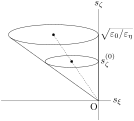
\includegraphics[scale=0.4]{scorn.pdf}
  \caption{}
  \label{scorn}
\end{figure}

% 直円錐(頂点から下した垂線の足と底面の円の中心が一致する円錐)を斜めに切って楕円が出てくるのとは別の話である.
さらに,$s$空間における点が実空間においてはベクトルになるように,$s$空間の平面は点$\boldsymbol{s}$の集合であり,実空間の平面になるとは限らないことに注意.
ある平面$s_\zeta=s_\zeta^{(0)}$でこの平面を切ると,これは底面と相似な円となり,$s_\zeta^{(0)}\sqrt{\varepsilon_\eta/\varepsilon_0}$倍になっている.
よって,円錐面の方程式は,
\begin{align*}
  \left(s_\xi+\dfrac{s_\zeta}{2}\sqrt{\dfrac{(\varepsilon_\zeta-\varepsilon_\eta)(\varepsilon_\eta-\varepsilon_\xi)}{\varepsilon_\xi\varepsilon_\zeta}}\right)^2+{s_\eta}^2=\left(\dfrac{s_\zeta}{2}\sqrt{\dfrac{(\varepsilon_\zeta-\varepsilon_\eta)(\varepsilon_\eta-\varepsilon_\xi)}{\varepsilon_\xi\varepsilon_\zeta}}\right)^2 .
\end{align*}
展開すれば,
\begin{align}
  {s_\xi}^2+\sqrt{\dfrac{(\varepsilon_\zeta-\varepsilon_\eta)(\varepsilon_\eta-\varepsilon_\xi)}{\varepsilon_\xi\varepsilon_\zeta}}s_\xi{}s_\zeta+{s_\eta}^2=0 . \label{biaxial_cornrot}
\end{align}
これを$\eta$軸に関して$-\beta$回転させると元の円錐が得られ,その変換は
\begin{align}
  \begin{split}
    s_\xi \to s_\xi\cos\beta-s_\zeta\sin\beta , \\
    s_\zeta \to s_\zeta\cos\beta+s_\xi\sin\beta .
  \end{split}
\end{align}
である.これを(\ref{biaxial_cornrot})に適用して,
\begin{align}
  (\varepsilon_\zeta-\varepsilon_\xi){s_\eta}^2 +
  \left[s_\xi\sqrt{\varepsilon_\xi(\varepsilon_\zeta-\varepsilon_\eta)} - s_\zeta\sqrt{\varepsilon_\zeta(\varepsilon_\eta-\varepsilon_\xi)}\right]
  \left(s_\xi\sqrt{\dfrac{\varepsilon_\zeta-\varepsilon_\eta}{\varepsilon_\xi}}-s_\zeta\sqrt{\dfrac{\varepsilon_\eta-\varepsilon_\xi}{\varepsilon_\zeta}}\right) = 0\label{biaxial_corn}
\end{align}
となる.この円錐面を内部円錐と呼ぶ.$\boldsymbol{s}$は$s$空間においてこの内部円錐と光線速度面の交線である円上に存在する.

以上が定量的な説明であったが,次にこれを定性的に考えよう.$\boldsymbol{s}$から光線速度面を使って$\boldsymbol{n}$を作る方法を使う.

\begin{figure}[ht]
  \centering
  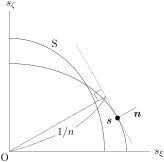
\includegraphics[scale=0.3]{ston.pdf}
  \caption{ $s$空間であることに注意}
  \label{ston}
\end{figure}

まず,ある$s$空間と光線ベクトル$\boldsymbol{s}$を考えよう.この空間内において$\boldsymbol{s}$は点として存在する.
今,媒質内のある点で$\boldsymbol{s}$が与えられた.この時,$s$空間に光線速度面方程式で決定される光線速度面Sを記入する.
そして,与えられた$\boldsymbol{s}$における法線を決定する.この法線の$s$空間における向きが屈折率ベクトル$\boldsymbol{n}$の実空間での向きと等しくなる.
図を見れば明らかなように,$\boldsymbol{s}$における光線速度面Sの接平面に原点から下した垂線はやはり$\boldsymbol{n}$の向きを向いている.
さらに,$\boldsymbol{s}\cdot\boldsymbol{n}$であることから,その長さは$\dfrac{1}{n}$である.

先程調べたように,2軸性異方性媒質の光線速度面上には同じ向きの法線を持つ領域が存在する.この点それぞれ$\boldsymbol{s}^{(1)}$, $\boldsymbol{s}^{(2)},\ldots$などと区別する.
ここで,任意の$\boldsymbol{s}^{(i)}$における接平面C$^{(i)}$を考える.この接平面は光線ベクトルに依らず,(\ref{biaxial_plane})で与えられる.
原点からこの平面に下した垂線の向きがこれに対応する$\boldsymbol{n}^{(i)}$の向きを定め,長さの逆数が$\boldsymbol{n}^{(i)}$の絶対値を与える.
また,C$^{(i)}$はOaと直交するので,先程述べた任意の$\boldsymbol{s}$に対する垂線は全てOaのことであると分かる.よって,これから
$\boldsymbol{s}^{(i)}$に対応する$\boldsymbol{n}^{(i)}$は全てOaであることが分かる.
この結果を実空間で書き直すと,
双法線方向の$\boldsymbol{n}$を持つ光の$\boldsymbol{s}$は(\ref{biaxial_corn})で決定され内部円錐(と同じ形をした円錐)の側面に存在することが分かる.
これを内部円錐屈折と言う.

同様に,双径線方向に$\boldsymbol{s}$があるとき,無限個の$\boldsymbol{n}$を考えることができる.これを
外部円錐屈折と言う.
同様の計算により,接平面は
\begin{align}
  n_\xi\sin\gamma+n_\zeta\cos\gamma=\sqrt{\dfrac{\varepsilon_\eta}{\varepsilon_0}}
\end{align}
で与えられ,外部円錐は,
\begin{align}
  \varepsilon_\eta(\varepsilon_\zeta-\varepsilon_\xi){n_\eta}^2+\left(n_\xi\sqrt{\varepsilon_\zeta-\varepsilon_\eta}-n_\zeta\sqrt{\varepsilon_\eta-\varepsilon_\xi}\right)\left(n_\xi\varepsilon_\xi\sqrt{\varepsilon_\zeta-\varepsilon_\eta}-n_\zeta\varepsilon_\zeta\sqrt{\varepsilon_\eta-\varepsilon_\xi}\right)
\end{align}
で与えられる.上の図ではOa$'$b$'$で表されている.

内部円錐屈折を観測するには,双法線に垂直な方向に切り出した媒質を使い,それに垂直入射させる.
入射する波は初めは$\boldsymbol{s}$と$\boldsymbol{n}$とともに一致しているが,$\boldsymbol{n}$が双法線方向なので,$\boldsymbol{s}$が内部円錐に沿って分かれる.
我々が観察するのは$\boldsymbol{s}$なので,光は媒質に入ると内部円錐に沿って屈折するように見える.

\begin{figure}[ht]
  \centering
  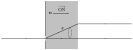
\includegraphics[scale=0.8]{innercornicalrefraction.pdf}
  \caption{双法線$(\protect\overrightarrow{\text{ON}})$向きの$\boldsymbol{n}$を持つ光は媒質に入ると内部円錐屈折を起こす}
  \label{innercornicalrefraction}
\end{figure}

外部円錐屈折を観測するには,双法線に垂直な方向に切り出した媒質を使い,それに垂直入射させる.ただし,この場合は,媒質の奥側にもスリットを置いておく.
媒質中を進むことができる光は$\boldsymbol{s}$が双径線方向の光のみである.この光の$\boldsymbol{n}$は外部円錐(図中に示した円錐)に沿って分布している.
媒質を出るときに光は屈折するが,屈折の時は群速度でなく波数が関係するのであった.2軸性媒質中と外部で,$\boldsymbol{n}$鉛直方向は変化しない.
よって,2軸性媒質を出た光はそれぞれ異なった$\boldsymbol{n}$を持つ.等方性媒質では$\boldsymbol{s}$と$\boldsymbol{n}$の向きが一致するので,媒質を出たのちの$\boldsymbol{s}$は円錐状に屈折する.
だが,$\boldsymbol{n}$の水平成分は屈折の際に変化するので,屈折後の$\boldsymbol{n}$は外部円錐に沿っていない.
そのため,$\boldsymbol{s}$も外部円錐には沿っていない.

\begin{figure}[ht]
  \centering
  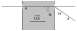
\includegraphics[scale=0.8]{outercornicalrefraction.pdf}
  \caption{外部で観測される光の向き$\boldsymbol{s}$は外部円錐と異なる}
  \label{outercornicalrefraction}
\end{figure}

円錐屈折は1832年に,W.R.Hamiltonが理論的に発見・予言し,後にH.Lloydが実験で確認した.
最近の研究で円錐屈折光からスロープ効率(定電流に対するレーザー強度)の高いレーザー発振が実現できることが分かり,レーザー結晶として使われたりする.
